%% copyright 2020 Dony Darmawan Putra & Hasan Albinsaid
 
\documentclass[12pt, twoside , openright]{book}

%%%%%%%%%% instant packages %%%%%%%%%%
%% Copyright 2020 Dony Darmawan Putra & Hasan Albinsaid

%% for dots table of contents

\usepackage{booktabs}
\usepackage{titletoc}% http://ctan.org/pkg/titletoc

\contentsmargin{0pt}
\renewcommand\contentspage{\thecontentspage}

\dottedcontents{section}[2.3em]{}{2.3em}{5pt}
\dottedcontents{subsection}[5.5em]{}{3.2em}{5pt}


 \titlecontents*{chapter}% <section-type>
  [0pt]% <left>
  {}% <above-code>
  {\bfseries\chaptername\ \thecontentslabel\quad}% <numbered-entry-format>
  {}% <numberless-entry-format>
  {\bfseries\dotfill\contentspage\\\vspace{0mm}}% <filler-page-format> 

 \titlecontents*{section}% <section-type>
  [0pt]% <left>
  {}% <above-code>
  {\bfseries\ \thecontentslabel\quad}% <numbered-entry-format>
  {}% <numberless-entry-format>
  {\bfseries\dotfill\contentspage\\\vspace{0mm}}% <filler-page-format> 
  
   \titlecontents*{subsection}% <section-type>
  [0pt]% <left>
  {}% <above-code>
  {\hspace{2mm}\bfseries\ \thecontentslabel\quad}% <numbered-entry-format>
  {}% <numberless-entry-format>
  {\bfseries\dotfill\contentspage\\\vspace{0mm}}% <filler-page-format> 

\newcommand*{\noaddvspace}{\renewcommand*{\addvspace}[1]{}}
\addtocontents{lof}{\protect\noaddvspace}
\addtocontents{lof}{\linespread{1}\selectfont}
\addtocontents{lot}{\protect\noaddvspace}
\addtocontents{lot}{\linespread{1}\selectfont}

%% Arabic Text
\usepackage[utf8]{inputenc}
\usepackage{arabtex}

%% for Chinese typing
\usepackage{xeCJK}
\setCJKmainfont{AR PL KaitiM Big5}                    

%% for sections
\usepackage{mfirstuc}

%% for times new roman
\usepackage{mathptmx}

%% for images
\usepackage{graphicx}
\graphicspath{ {Images/} }
\usepackage{caption}
\usepackage{subcaption}

%%  for paper size and margins
\usepackage[a4paper,top=2.54cm,bottom=2.54cm, left=3cm, right=3cm]{geometry}


%% for paragraph
%paragraph indentation
\usepackage{indentfirst}
\setlength{\parindent}{4em} 

%paragraph spacing
\setlength{\parskip}{1em}

%Line spacing
\renewcommand{\baselinestretch}{2}

%% for font size
\usepackage{setspace}
\usepackage{blindtext}
\newcommand{\bigsize}{\fontsize{16pt}{20pt}\selectfont}
\newcommand{\chinnesesize}{\fontsize{18pt}{20pt}\selectfont}

%% for header and footer
\usepackage{blindtext}
\pagestyle{plain}


%% for references
\usepackage[square,numbers]{natbib}
\renewcommand{\bibsection}{}

%% for chapter title
 \usepackage{titlesec}
 \titleformat{\chapter}[display]{}{\filright  \LARGE  \chaptername\enspace\thechapter}{-2pt}{\filright\LARGE  \bfseries}[\vskip0pt]
 \titleformat{name=\chapter, numberless}{}{}{-10pt}{\filright \enspace}[\vskip0pt]

 \titlespacing{\chapter}{-20pt}{-20pt}{10pt}
 \titlespacing{name=\chapter, numberless}{-10pt}{-10pt}{-10pt}
 
\titlespacing*{\section}
{0pt}{0pt}{0pt}
\titlespacing*{\subsection}
{0pt}{0pt}{0pt}
 
\renewcommand{\contentsname}{\hfill\bfseries\LARGE Table of Contents \hfill}
\renewcommand{\listfigurename}{\hfill\bfseries\LARGE Table of Figures \hfill}
\renewcommand{\listtablename}{\hfill\bfseries\LARGE Table of Tables \hfill}
  

%% Algorithm    
\usepackage{algorithmic}
\usepackage[utf8]{inputenc}
\usepackage{amsmath,amssymb,amsfonts}
\usepackage{mathtools}
\usepackage[ruled,vlined,algochapter]{algorithm2e}
\usepackage{varioref}
\usepackage{hyperref}


%% Math Set Symbol
\usepackage{newtxmath}

%%%%%%%%%%%%%%%%%%%%%%%%%%%%%%%%%%%%%%%%
%%%%%%%%%% for body of document %%%%%%%%%%
%%%%%%%%%%%%%%%%%%%%%%%%%%%%%%%%%%%%%%%%
\begin{document}

%%%%%%%%%% cover %%%%%%%%%%
\thispagestyle{empty}
\begin{center}
	\onehalfspacing
	
\includegraphics[width=0.205\textwidth]{logo_nsysu_thesis}
	
	{\chinnesesize 國立中山大學 Your Departement Chinese Name %%NSYSU Your Departement Name
		
		碩士論文} %%Master Thesis
	
	{\bigsize Your Departement Name\\National Sun Yat-sen University\\}
	{\bigsize Master Thesis\\}
	
	\vspace{2cm}
	{\chinnesesize Chinese Thesis Title\\}
	{\bigsize Thesis Title\\}
	\vspace{2cm}
	{\bigsize 研究生:Your Chinese Name\\
		\hspace{70pt} Your Name\\
		指導教授:Advisor Chinese Name\\
		\hspace{130pt}Advisor Name \\
	}
	
	\vspace{1.5cm}
	
	{\bigsize 中華民國109年1月\\
		January 2020\\
		
	}
\end{center}

\newpage
\mbox{}
\thispagestyle{empty}
\newpage
\pagenumbering{roman}


%%%%%%%%%% for thesis Validation Letter %%%%%%%%%%
\addcontentsline{toc}{chapter}{Thesis Validation Letter}
\begin{center}
	{\chinnesesize Thesis Validation Letter }
\end{center}
Validation letter
\newpage
\mbox{}
\newpage


%%%%%%%%%% acknowledgment %%%%%%%%%%
\addcontentsline{toc}{chapter}{Acknowledgements}
\begin{center}
	{\chinnesesize Acknowledgements}
\end{center}
\setarab
\fullvocalize
\arabtrue
\begin{center}
	\begin{RLtext}
		bismi al-ll_ahi al-rra.hm_ani al-rra.hImi
	\end{RLtext}
\end{center}

Alhamdulllahirabbil’alamin, finally got to this point, a splash of success that You gave me Rabb Allah SWT is the Almighty, endlessly thanking you. Prayers and greetings to the Prophet Muhammad SAW and his noble friends.  

In accordance with the words of the Prophet Muhammad SAW that when we have an advantage we might help the other people, as mentioned in hadith narrated by Ath-Thabrani:

\begin{center}
	\begin{RLtext}
		a.habba Al-nnaasi 'il_A al-ll_ahi ta`aa l_A aanfa`uhum lil-nnaasi..
	\end{RLtext}
\end{center}


"The most loved Man/Woman by Allah is the most beneficial to humans  beings.." (Narrated by Ath-Thabrani in Al Mu’jam Al Kabir no. 13280).

Hopefully, this NSYSU Thesis LaTEX template can be useful for all of us, and you'll get the best results for your thesis.

\noindent
Author :

\vspace{-2em}
- Dony Darmawan Putra

\vspace{-2em}
- Hasan Albinsaid

\newpage
\mbox{}
\newpage





%%%%%%%%%% chinnese abstract %%%%%%%%%%
\addcontentsline{toc}{chapter}{摘 要}
\begin{center}
	{\chinnesesize 摘 要}
\end{center}
This is Abstract, but in chinese language. \blindtext[1]
\newpage
\mbox{}
\newpage





%%%%%%%%%% english abstract %%%%%%%%%%
\addcontentsline{toc}{chapter}{Abstract}
\begin{center}
	{\chinnesesize Abstract}
\end{center}

This is Abstract. \blindtext[1]

\noindent Keywords: keyword1, keyword2, keyword3.
\newpage




%%%%%%%%%%
\tableofcontents
\newpage




%%%%%%%%%%
\listoffigures
\newpage




%%%%%%%%%%
\listoftables
\newpage




%%%%%%%%%%%%%%%%%%%%%%%%%%%%%%%%%%%%%
%%%%%%%%%%for Main Contents%%%%%%%%%%
%%%%%%%%%%%%%%%%%%%%%%%%%%%%%%%%%%%%%
\mainmatter

%%%%%%%%%%First Chapter%%%%%%%%%%
\chapter{Introduction}
This is your introduction. You can put the citation as this example \cite{CpLi}. For adding reference you can open bibliography file "references.bib" and paste the BibTeX into that file, to make it more clear you can see the example of BibTex in this link : \href{https://www.youtube.com/watch?v=SsJSR2b4_qc&t=107s}{Import BibTeX from Google Scholar}

 \blindtext[2] %<-this is dummy text





%%%%%%%%%%Second Chapter%%%%%%%%%%
\chapter{Second Chapter}
This is your second chapter, the example for citation \cite{Ymc}. \blindtext[1]

You can add figure, so it will show as Figure \ref{fig:figure_ref}
\begin{figure}[h]
	\centerline{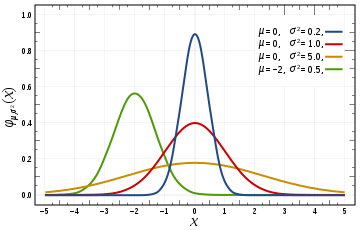
\includegraphics[width=0.5\columnwidth]{Images/gambar.png}}
	\caption{Gaussian distribution1}
	\label{fig:figure_ref}
\end{figure}


\section{Sub chapter}\label{sub_chapter21}
This is your sub chapter, the example for citation \cite{latexcompanion}. \blindtext[1].
\begin{equation}
\label{index_eq}
(\hat{n})=\operatorname*{arg\,max}_{n\in \{1,\dots,M\}}(\mathbf{X}_{n})
\end{equation}
This is the example of equation, expressed as eq. \ref{index_eq}

\SetKwInput{KwInput}{Input}
\SetKwInput{KwOutput}{Output}  
\begin{algorithm}
	%\DontPrintSemicolon
	\KwInput{$\mathbf{A}$,$\mathbf{B}$}
	\For{$j\gets1$ to $N_s$ by $1$}{
		\For{$i\gets1$ to $N$ by $1$}{
			$\mathbf{A}[i,j]=i+j$
		}
	}
	$\mathbf{C}=\mathbf{A}+\mathbf{B}$
	
	\KwOutput{Matrix result $\mathbf{C}$ }
	\caption{The example of algorithm}
\end{algorithm}


\section{Sub chapter}\label{sub_chapter22}
This is your sub chapter. \blindtext[2]
\begin{figure}[h]
	\centerline{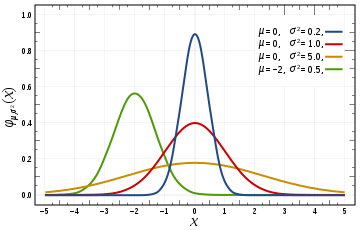
\includegraphics[width=0.5\columnwidth]{Images/gambar.png}}
	\caption{Gaussian distribution2}
	\label{fig:figure_ref2}
\end{figure}




%%%%%%%%%%Third Chapter%%%%%%%%%%
\chapter{Third Chapter}
This is your third chapter. \blindtext[1] 

\section{Sub chapter}\label{sub_chapter31}
This is your sub chapter. \blindtext[1] You can add table, so it will show as Table \ref{table:table1}

\begin{table}[h!]
	\begin{center}
		\caption{This is the example of table1}
		\label{table:table1}
		\begin{tabular}{|l|c|c|c|}
			\hline
			\textbf{Layer} & \textbf{Col1} & \textbf{Col2} \\ % <-- added & and content for each column
			\hline
			Row1 & content & content \\ % <--
			Row2 & a & b \\ % <--
			Row3 & c & d \\ % <--
			Row4 & e & f \\ % <--
			\hline
		\end{tabular}
	\end{center}
\end{table}

\section{Sub chapter}\label{sub_chapter32}
This is your sub chapter. \blindtext[2]
\begin{table}[h!]
	\begin{center}
		\caption{This is the example of table2}
		\label{table:table2}
		\begin{tabular}{|l|c|c|c|}
			\hline
			\textbf{Layer} & \textbf{Col1} & \textbf{Col2} \\ % <-- added & and content for each column
			\hline
			Row1 & content & content \\ % <--
			Row2 & a & b \\ % <--
			Row3 & c & d \\ % <--
			\hline
		\end{tabular}
	\end{center}
\end{table}




\chapter{Conclusion}
The conclusion is... \blindtext[1] %<-this is dummy text
\newpage
\mbox{}
\newpage



%% for Reference
\addcontentsline{toc}{chapter}{Reference}
\begin{center}
	{\chinnesesize Reference}
\end{center}
\bibliographystyle{IEEETran}
\bibliography{references}

\newpage
\mbox{}
\newpage

\end{document}
